\chapter{Implementation} \label{chapter:implementation}
The tools implemented include exploration of datasets using statistical overviews and visualizations, experiments of feature selection which involve machine learning pipeline, and firmware for data logger's hardware. 

\section{Data analysis}
The data processing and data mining on the MaFaulDa and Pump dataset takes place in several \emph{JupyterLab} notebooks written in \emph{Python} language. The purpose of individual notebooks is described in detail in Appendix~\ref{appendix:technical-docs}. Utility functions are located in separate package \emph{vibrodiagnostics} so that the experiments can be realized under multiple conditions.

The tabular data is handled using \emph{Pandas}dataframes that are training batch models from \emph{scikit-learn} library and \emph{imbalanced-learn}, or online models from \emph{RiverML}. The wide variety of graphs and other visualizations are stylized with \emph{Matplotlib} and \emph{Seaborn}. Feature calculation is crafted according to mathematical formulas atop libraries \emph{Numpy}, \emph{SciPy}, and \emph{Time Series Feature Extraction Library}~(TSFEL).

\begin{lstlisting}[style=pythonstyle,caption=Rank product of feature matrix X to label column Y,label={lst:rank-product},morekeywords={DataFrame,rank,set_index,sort_values,gmean}]
METRICS = {
    "corr": selection.corr_classif, 
    "f_stat": sklearn.feature_selection.f_classif, 
    "mi": sklearn.feature_selection.mutual_info_classif }
r = pandas.DataFrame()
for name, metric in METRICS.items():
    # Order the features to leaderboard
    r[name] = leaderboard  
ranks = r.rank(axis="rows", method="first", ascending=False)
return ranks.apply(scipy.stats.gmean, axis=1).sort_values()
\end{lstlisting}

\begin{lstlisting}[style=pythonstyle,caption=Leaderboard of feature importance metric scores,label={lst:feature-leaderboard},morekeywords={DataFrame,rank,set_index,sort_values,metric,gmean}]
pandas.DataFrame(zip(X.columns, metric(X, Y)), 
                 columns=["feature", "score"])
      .set_index("feature")
      .sort_values(by="score", ascending=False))
\end{lstlisting}

Since the central focus of this work targets feature selection, the source code listing~\ref{lst:rank-product} and \ref{lst:rank-product} demonstrates the ranking scores calculated for features in data frame X. Leaderboards are united by geometric mean to produce rank product ordering.

\section{Firmware}
The drivers for low-level interfaces of ESP32 microcontroller and FAT32 filesystem are already available in Espressif ESP-IDF SDK. The accelerometer driver is made available by the vendor\footnote{IIS3DWB driver: \url{https://github.com/STMicroelectronics/iis3dwb-pid}}. The entry routine of the firmware mounts the SD card, sets up GPIO pins for LED and button, and executes three \emph{FreeRTOS} tasks. Procedures in firmware are described in Appendix~\ref{appendix:technical-docs}. The hardware (Fig.~\ref{fig:hw-data-logger}) was built by the thesis consultant based on the complete specification supplied by the author.

\begin{figure}[h]
    \centering
    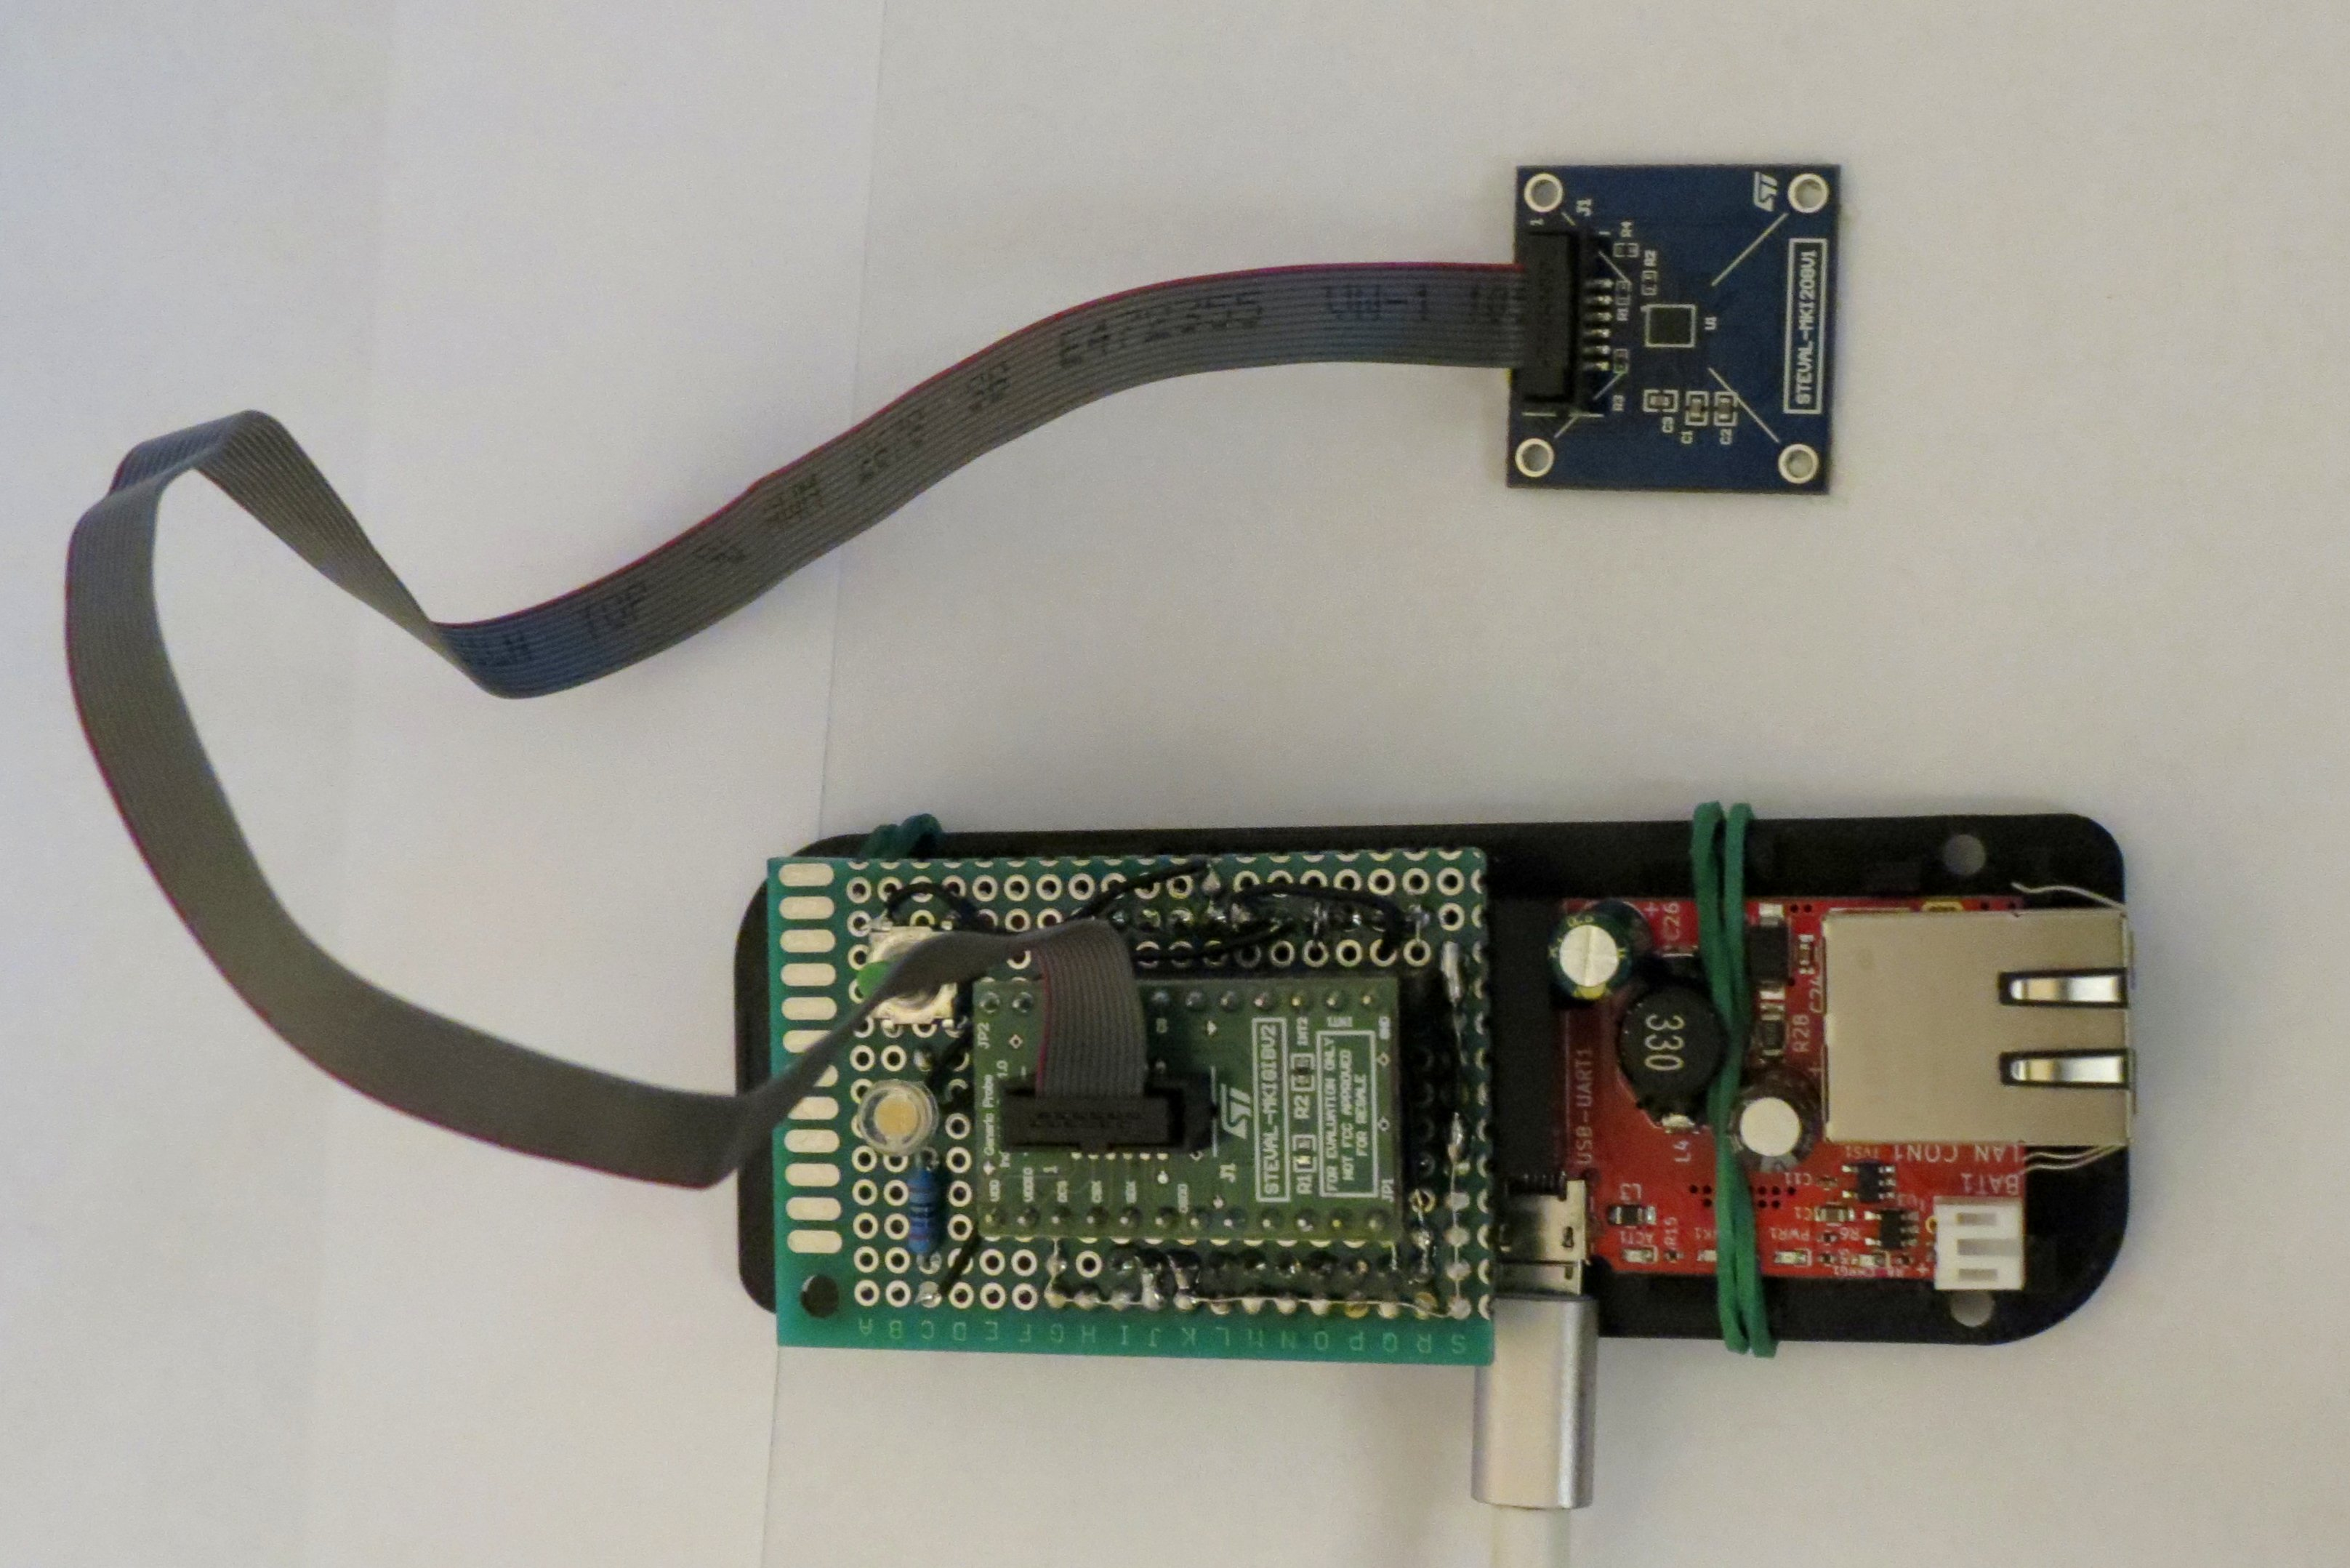
\includegraphics[width=0.7\textwidth]{assets/design/sensor/data-logger.jpg}
    \caption{Accelerometer Data Logger}
    \label{fig:hw-data-logger}
\end{figure}

The tasks run on an event-driven basis through notifications and a queue. They have the following purposes:
\begin{itemize}
\itemsep0pt
\item \textbf{Trigger task} - reacts to notification from button's interrupt handler. Depending on whether the recording is in progress, it either starts peripherals and creates a file or stops them and closes the file. Button debouncing has the form of a two-second delay when interrupts are ignored. The task is pinned to core 1 with priority 2 (higher numbers have more priority).
\item \textbf{Read task} - waits for notification from 9 ms periodic timer to read around half of the accelerometer's FIFO via half-duplex SPI bus at 8 MHz. It sends read-out samples to the queue. In case of any buffer overrun, it turns off the LED prematurely. The task is pinned to core 0 with priority 1.
\item \textbf{Write task} - reads the samples from the queue, and after locking the mutex for the opened file, it writes them to the card. The file is also manipulated within the trigger task, so the lock prevents race conditions. The task is pinned to core 1 with priority 1.
\end{itemize}

The testing process of the firmware revealed two issues that were resolved subsequently. The STEVAL evaluation board is plagued with broken hardware interrupt lines. The FIFO watermark interrupt on the INT1 pin of the accelerometer stopped firing after a few seconds and stayed at a high logic level. We noted the problem first on the digital multimeter, then confirmed it on an oscilloscope and found the same issue in the vendor's forum thread\footnote{IIS3DWB Interrupt stops triggering while sampling for long periods: \url{https://community.st.com/t5/mems-sensors/iis3dwb-interrupt-stops-triggering-while-sampling-for-long/td-p/203630}}.

\begin{figure}[h]
    \centering
    \begin{subfigure}[b]{0.49\textwidth}
        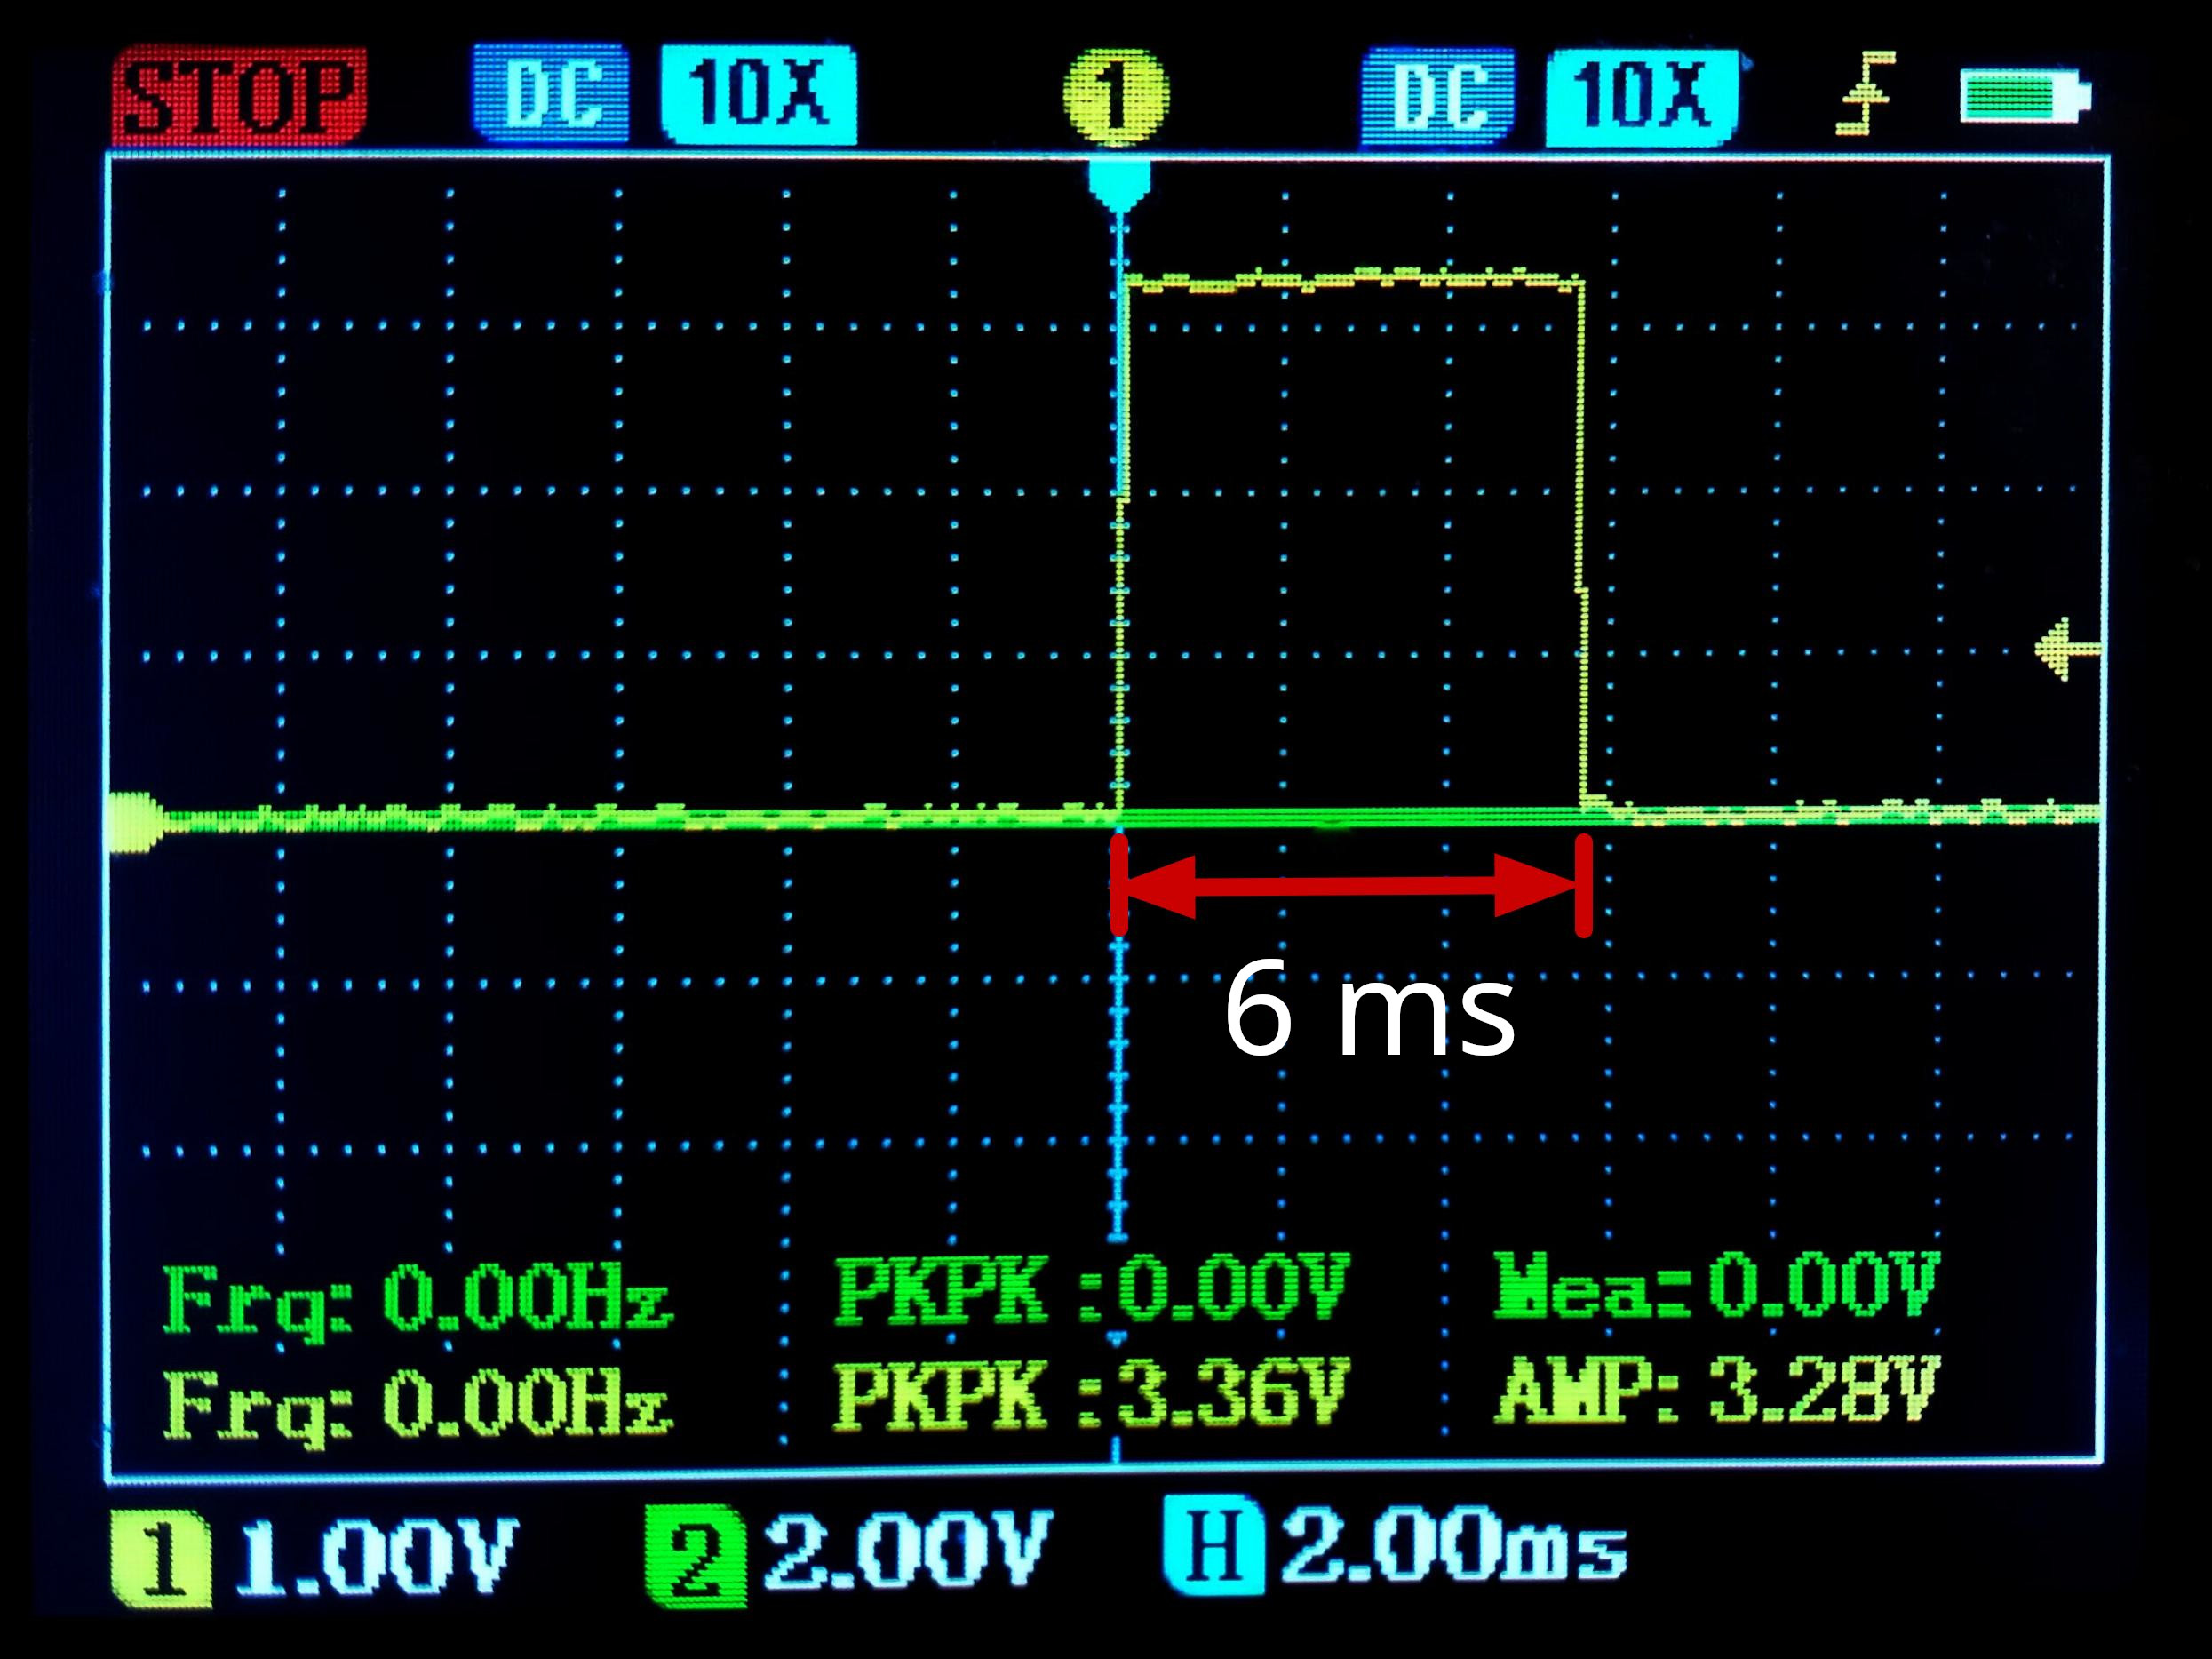
\includegraphics[width=\textwidth]{assets/design/oscilloscope/bin-fomat.jpg}
        \caption{Binary format}
        \label{fig:implementation:binary-format}
    \end{subfigure}
    \hfill
    \begin{subfigure}[b]{0.49\textwidth}
        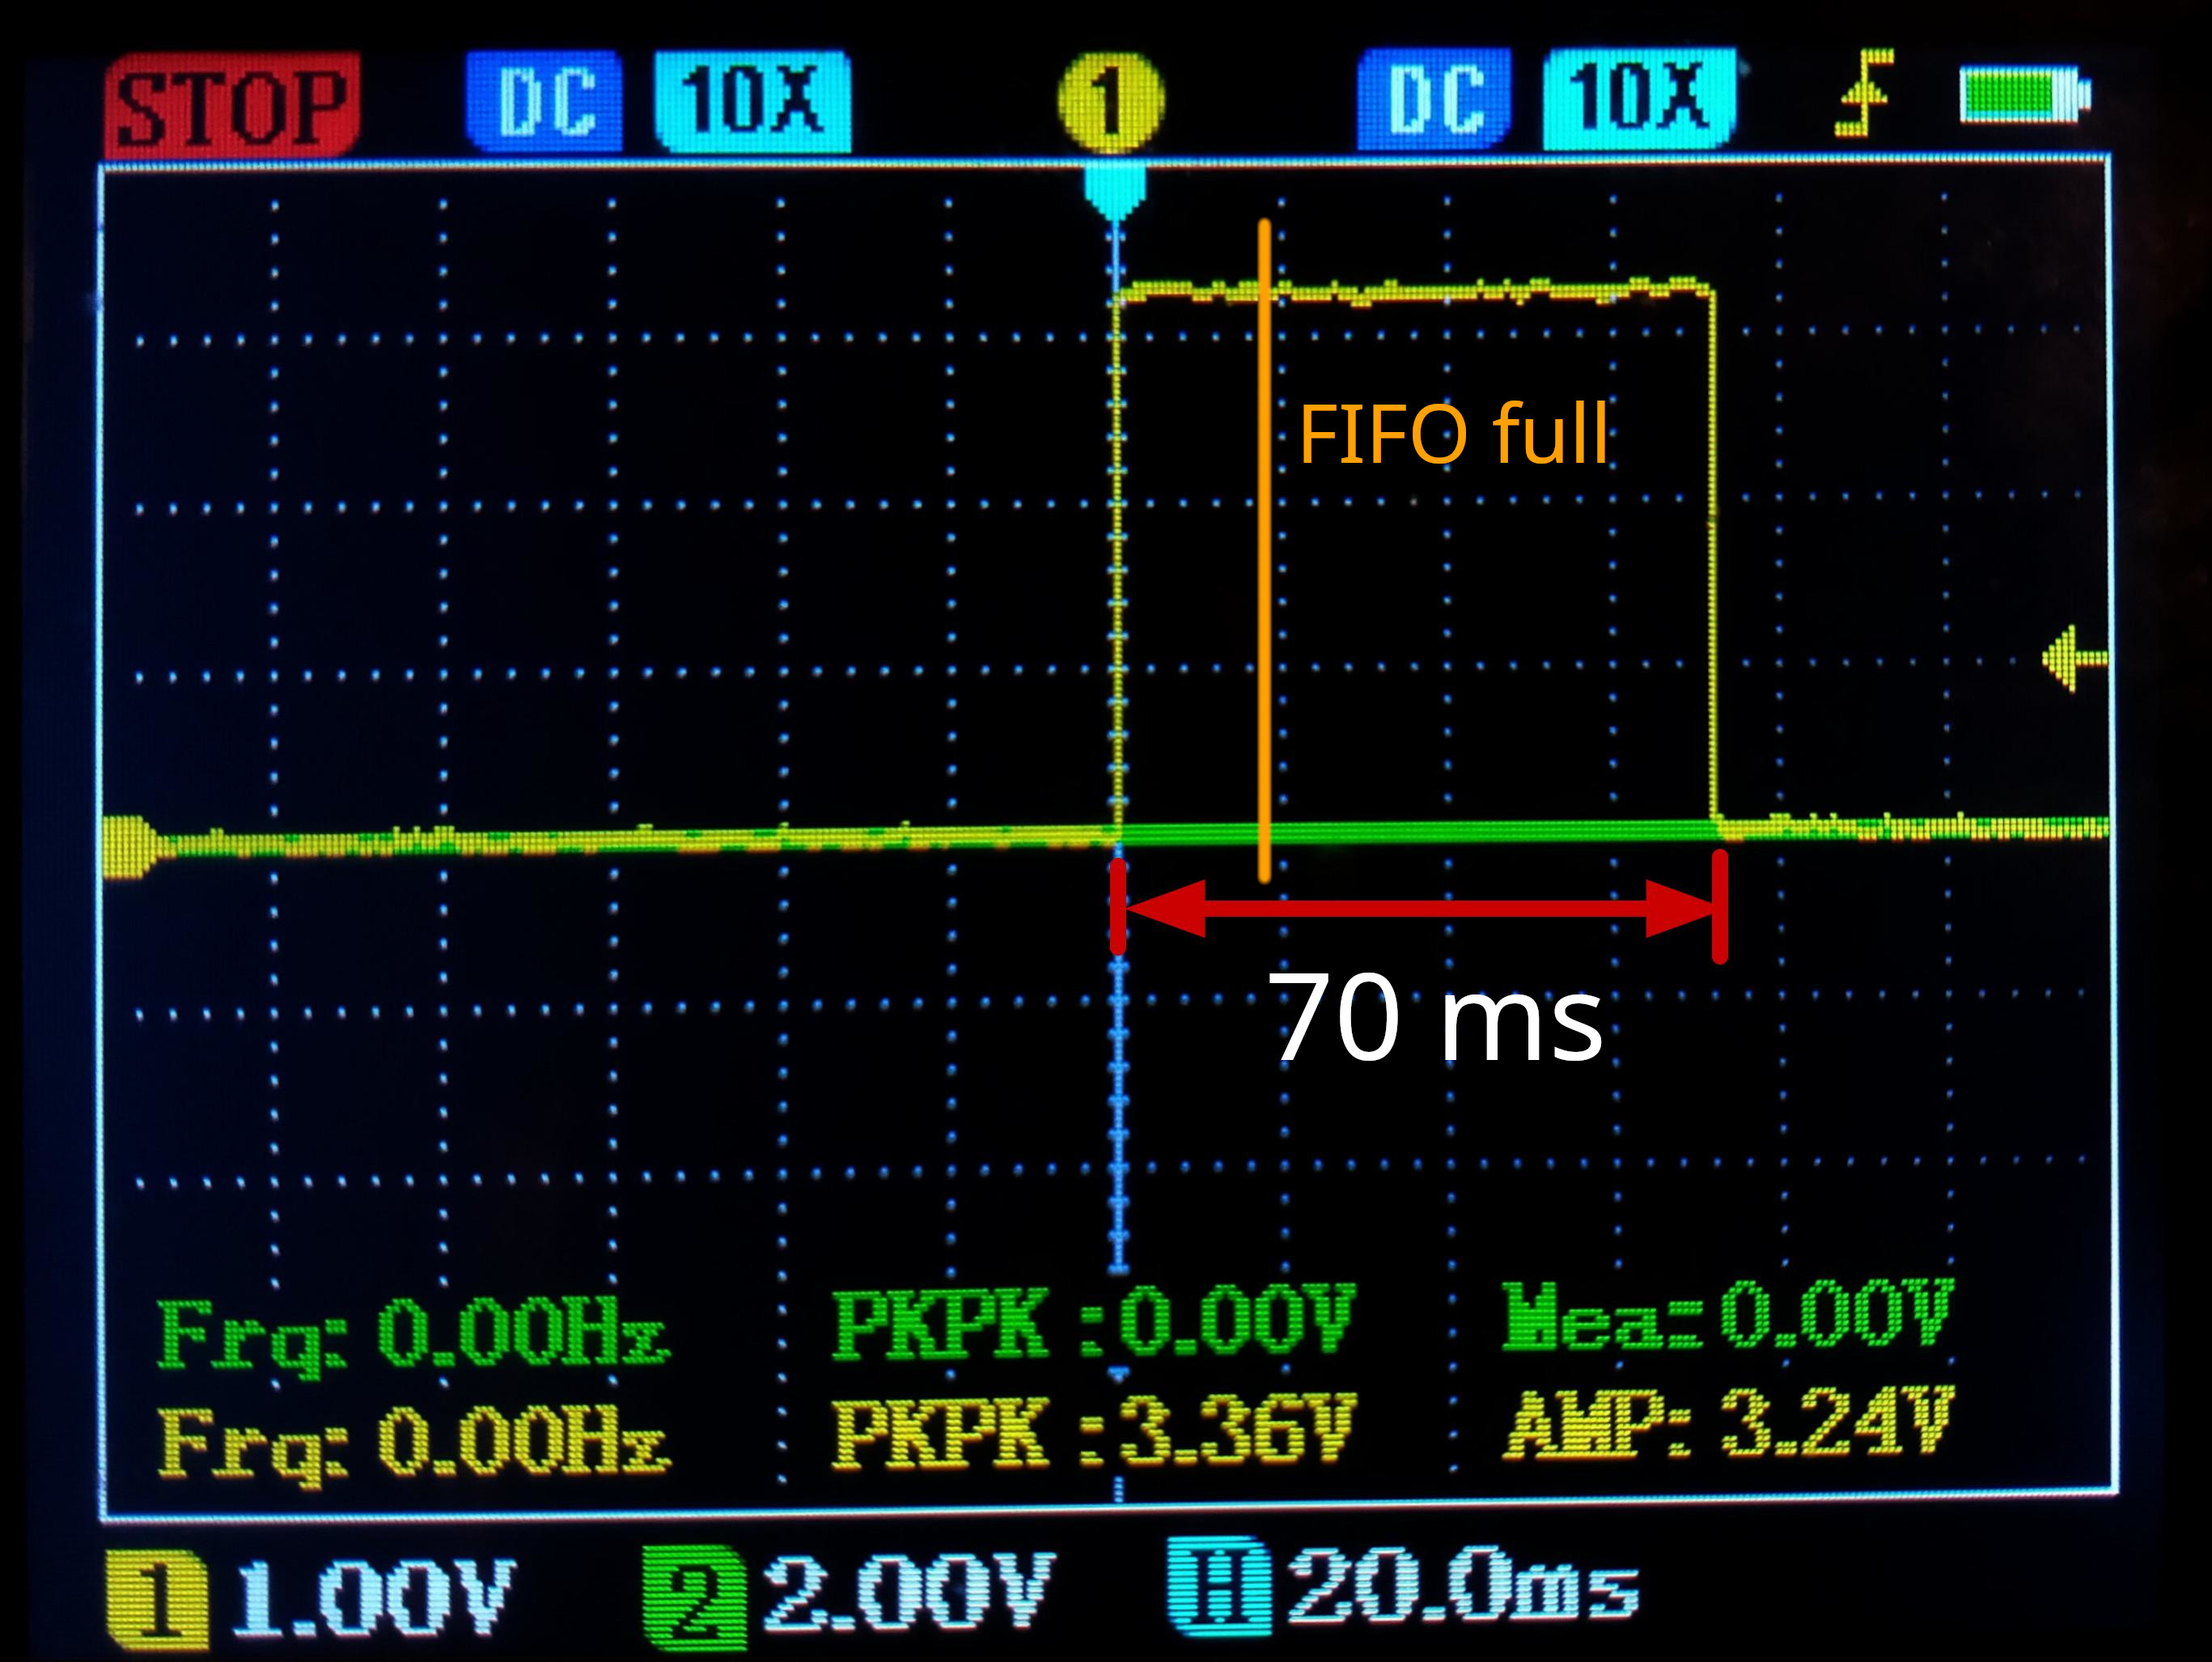
\includegraphics[width=\textwidth]{assets/design/oscilloscope/tsv-format.jpg}
        \caption{TSV format}
        \label{fig:implementation:tsv-format}
    \end{subfigure}
    \caption{Timing issue of writing samples to SD card captured on oscilloscope}
    \label{fig:implementation:file-write}
\end{figure}

Another impediment presented the slow string formatting with \emph{printf} family of functions during the accelerometer sampling. The readings cannot be written to TSV directly because the real-time (RT) deadline is not met due to the high sampling rate. It is true even if the queue is utilized and the processing takes place in another task. The binary files from the SD card are converted in bulk to TSV with custom Python command line script \verb|bin2tsv.py|.

During debugging, the pin was set to change the output level immediately before the one buffer started file write and after its completion. The scopes in Figure~\ref{fig:implementation:file-write} show the time the write took for binary compared to the TSV format. In writing to TSV format, the relation of numbers of already processed buffers $x$ to those left to process $y$ is: $y = 3.7x$. It is a monotonically increasing function, so the system would eventually overrun any sized assigned queue.

The hardware FIFO of 512 sample vectors fills up in 19.05 ms. The processing time $t$ has to satisfy inequality for deadline: $t \leq 2 \cdot \frac{1}{f_s} \cdot N_{FIFO} $. The RT deadline is 38.1 ms, beyond which the samples get dropped. In an embedded device, the short recoding burst (80.4 kSps) would need to be written temporarily in binary format to external memory and processed in two passes.

\begin{figure}[h]
    \centering
    \begin{subfigure}[b]{0.49\textwidth}
        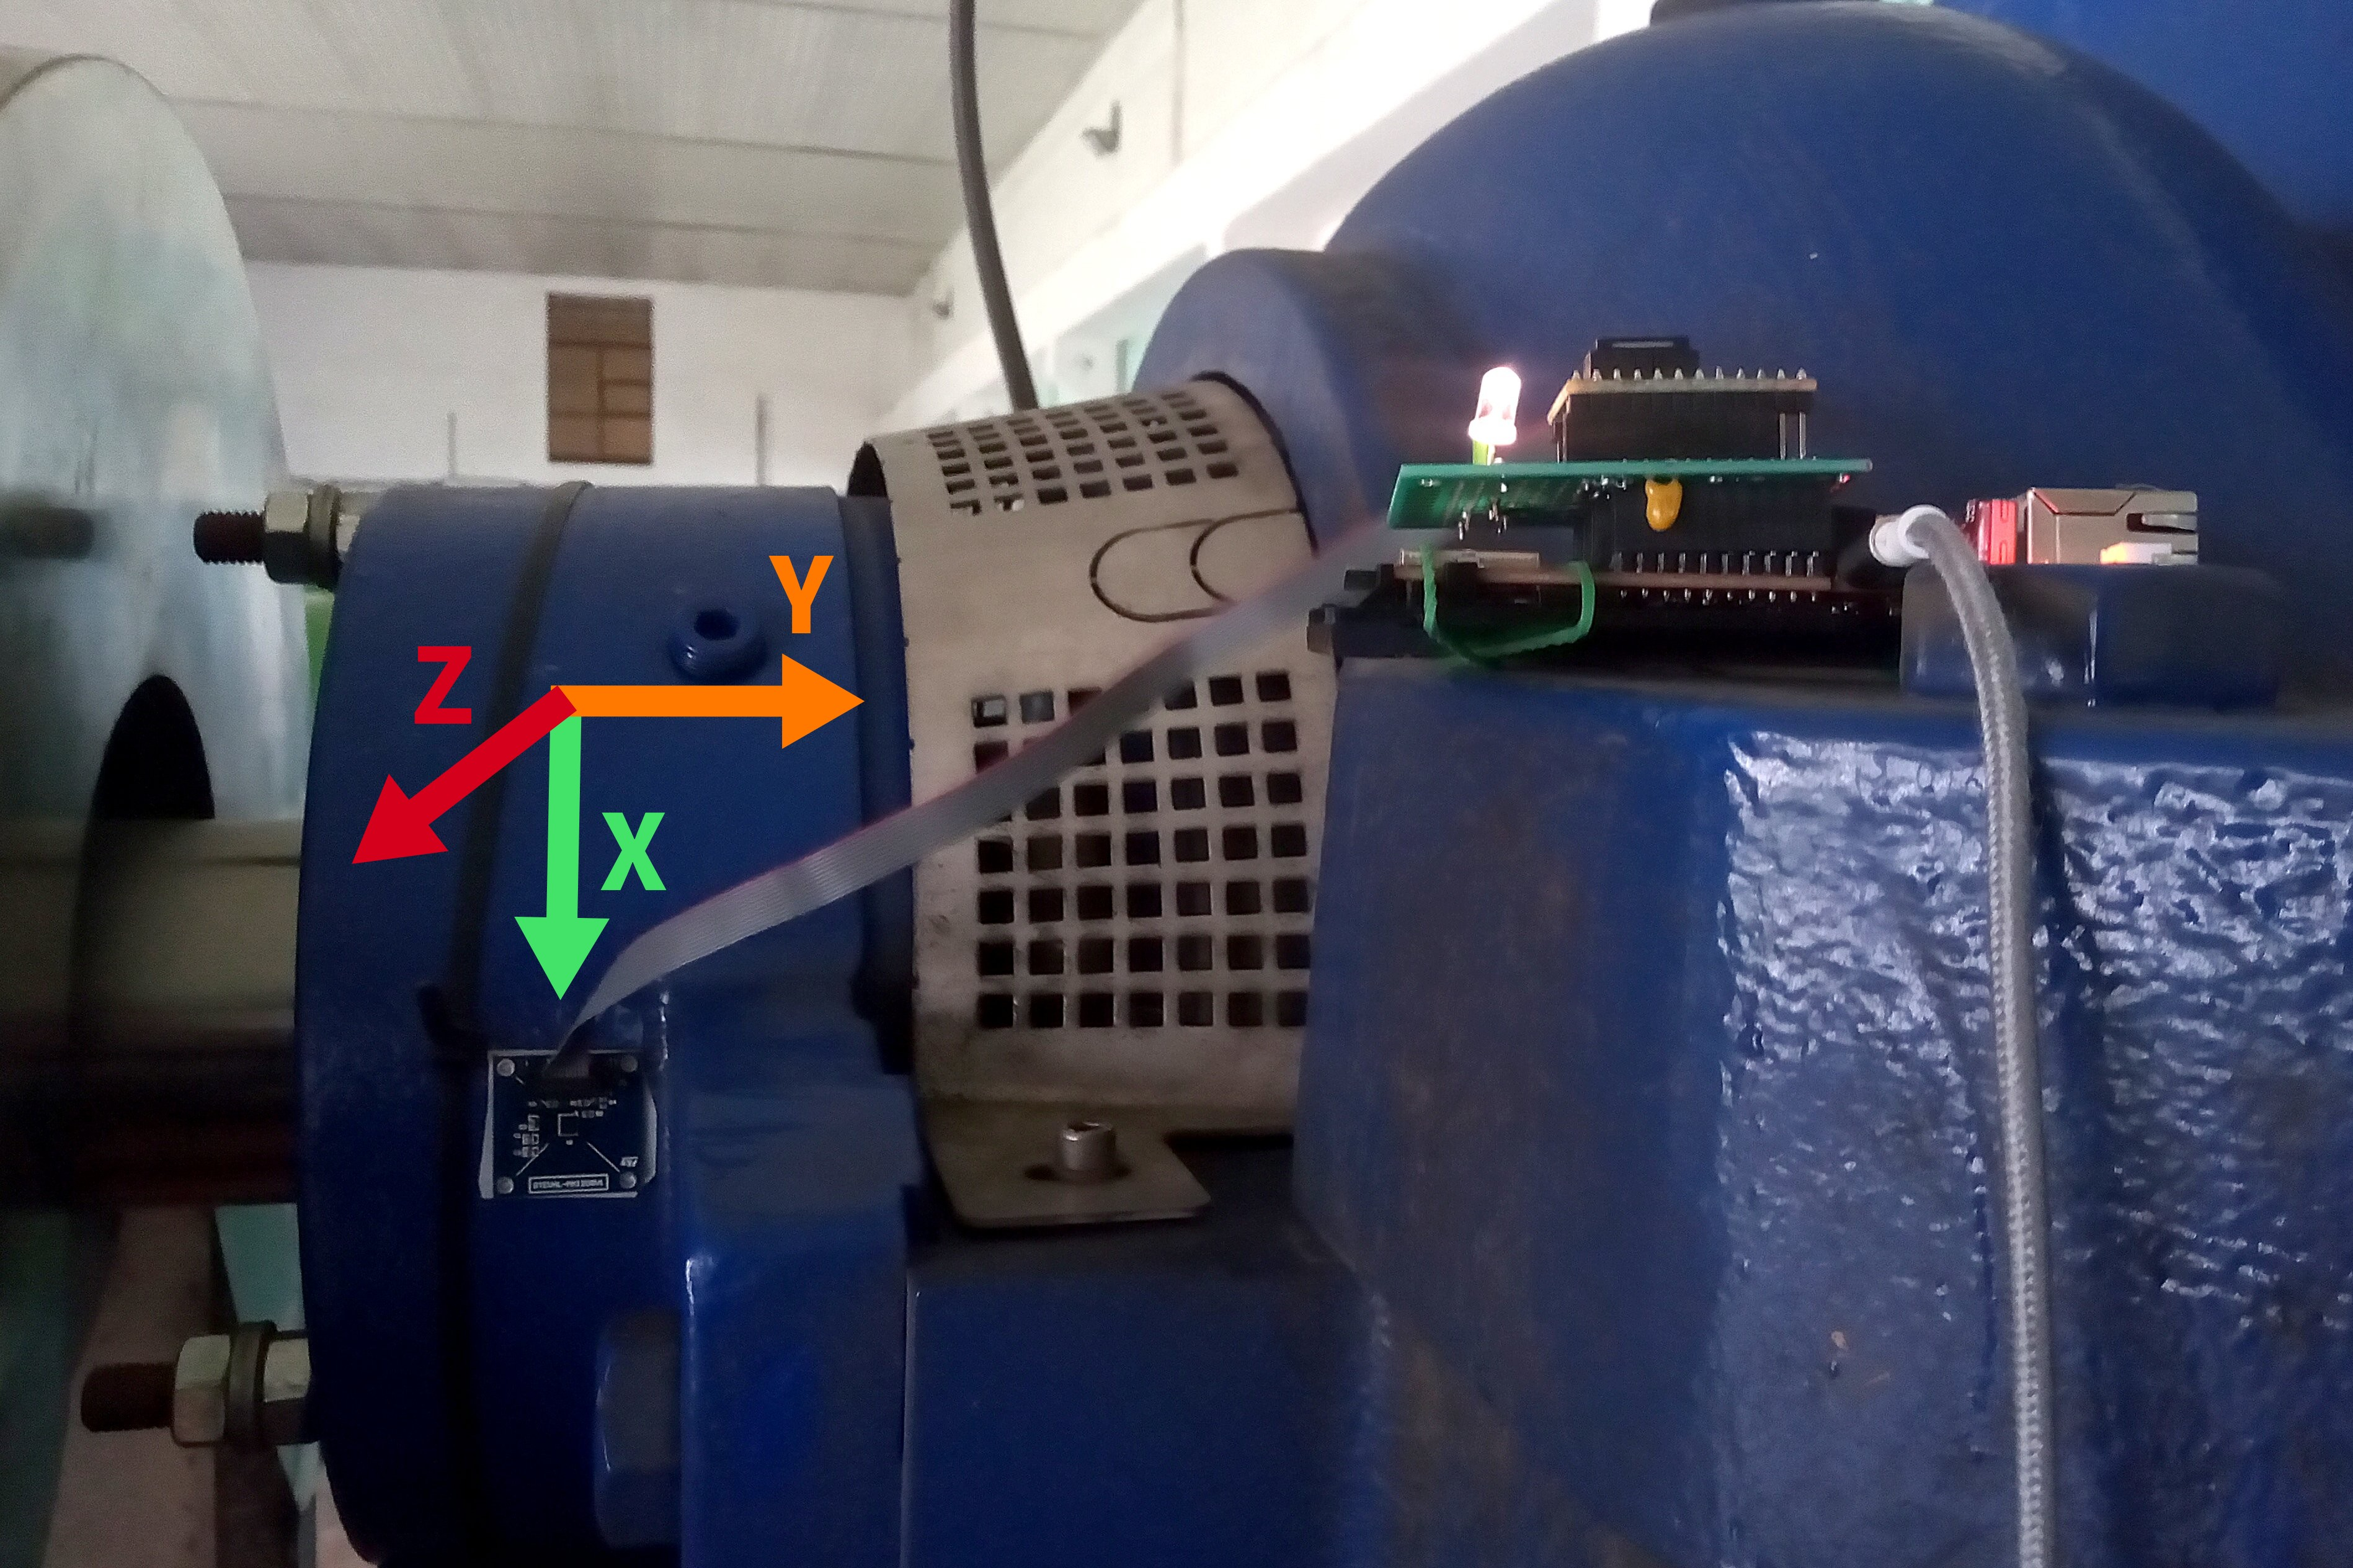
\includegraphics[width=\textwidth]{assets/design/sensor/sensor.jpg}
        \caption{Sensor on water pump}
    \end{subfigure}
    \hfill
    \begin{subfigure}[b]{0.49\textwidth}
        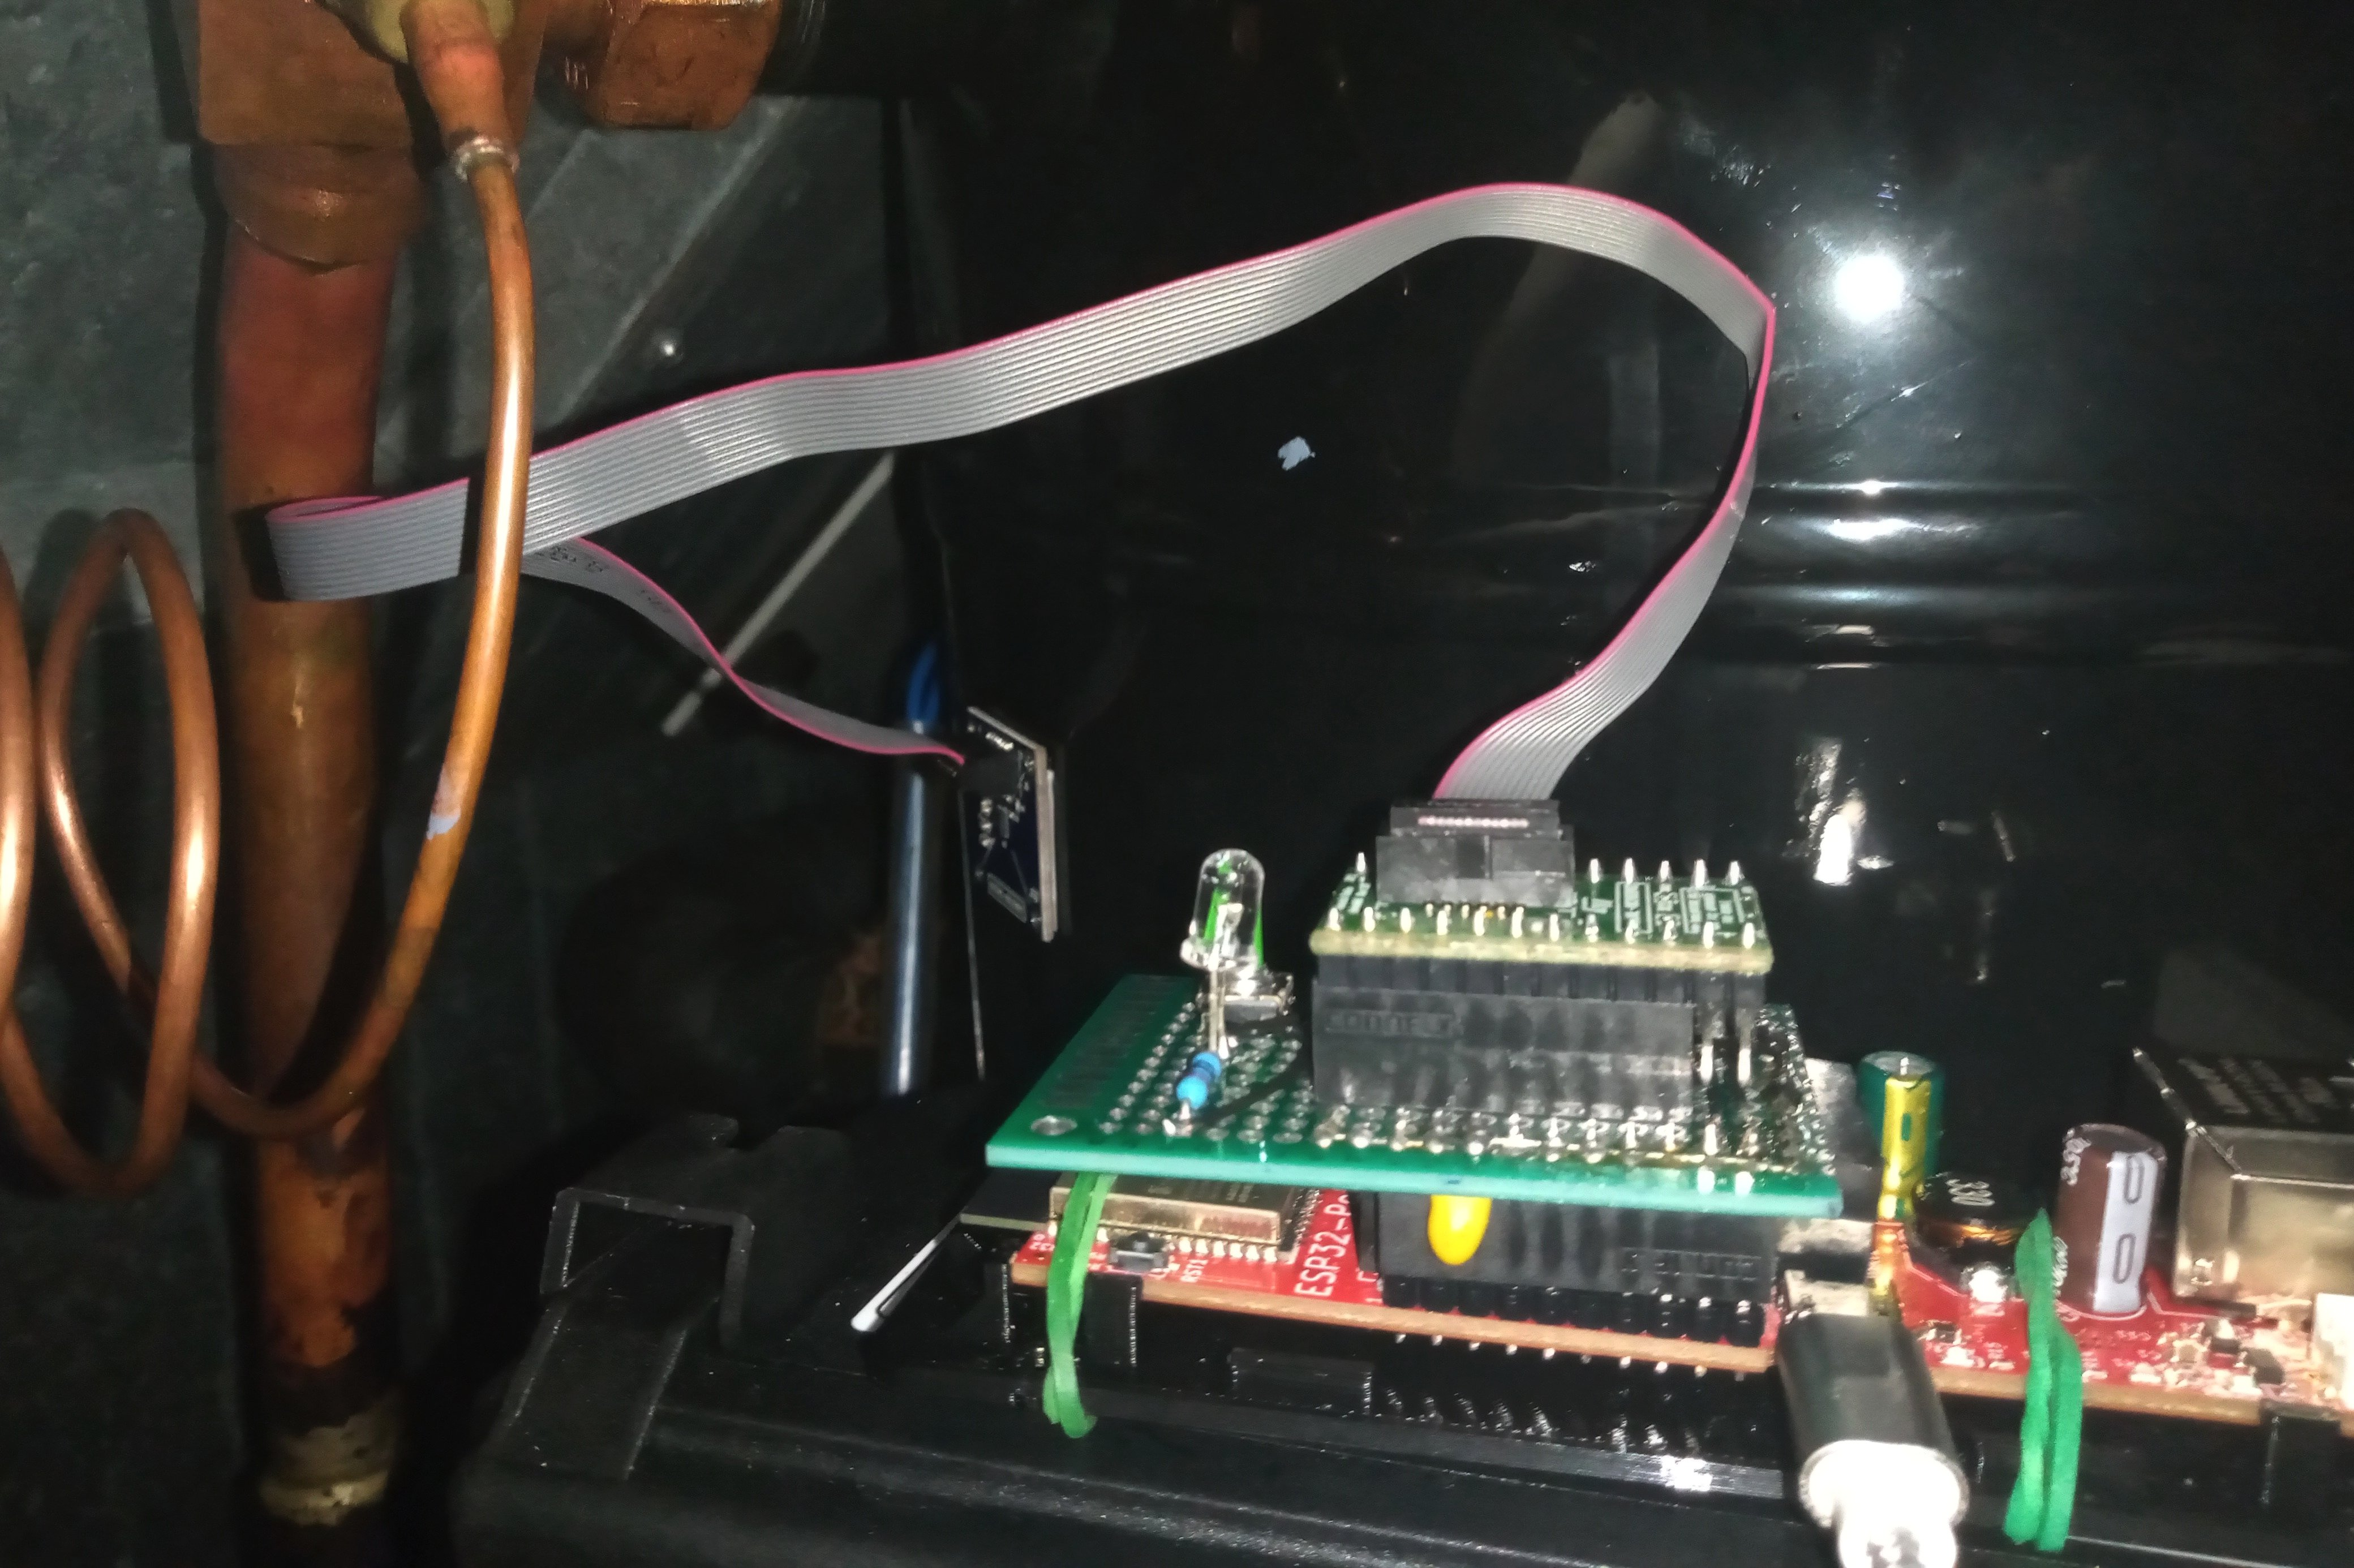
\includegraphics[width=\textwidth]{assets/design/sensor/sensor-compressor.jpg}
        \caption{Sensor on scroll compressor}
    \end{subfigure}
    \caption{Data logger on the machines in measurement positions}
    \label{fig:implementation:sensor-on-machine}
\end{figure}

Measurement conditions in the industry and axis orientation of the accelerometer are depicted in Figure~\ref{fig:implementation:sensor-on-machine}. The sensor is attached in tape to machines with a connector facing up and is pressed gently toward the surface.